\documentclass{article}
\usepackage[paperwidth=4cm,paperheight=6.9cm,left=0pt,right=0pt,top=0pt,bottom=0pt]{geometry}
\usepackage[utf8]{inputenc}
\usepackage[T1]{fontenc}
\usepackage{tikz}
\usetikzlibrary{decorations.pathmorphing,fadings}
\pagestyle{empty}
\begin{document}
\centering%
\tikzfading[name=topbottom, top color=transparent!0, bottom color=transparent!100]
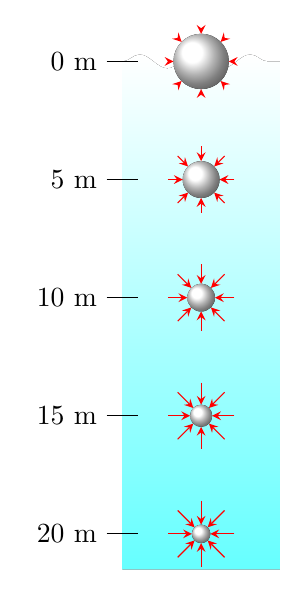
\begin{tikzpicture}[y=3mm]
\fill[draw=none,bottom color=cyan!60, top color=white] decorate[decoration=snake, segment length=20]{(0,0) -- (2,0)} -- ++(0,-21.5) -- (0,-21.5) -- cycle;
\foreach \y/\v in {0,5,...,20}
{
  \pgfmathparse{10 / (1 + \y/10)}\let\v\pgfmathresult
  \draw (-2mm,-\y) -- ++(4mm,0) node[pos=0,anchor=east]{\y~m};
  \fill[ball color=white] (1,-\y) circle (\v pt);
  \foreach \r in {0,45,...,315}
    \draw[-stealth,red] (1,-\y) +(\r:12pt) -- +(\r:\v pt);
}
\end{tikzpicture}%
\end{document}
